\documentclass[class=article , crop=false, titlepage, twoside, multi={itemize, figure, verbatim}, float=false]{standalone}

\usepackage{import} % Required for importing other .tex docs.  (import uses everything bw Begin and End Doc)
\usepackage{float} % Required for specifying the exact location of a figure or table
\usepackage{graphicx} % Required for including images
\usepackage{wrapfig}
\usepackage[pdftex,breaklinks,colorlinks=true,linkcolor=black,citecolor=blue,urlcolor=red,linktocpage=false,pagebackref=true,filecolor=magenta]{hyperref}%http://www.tug.org/applications/hyperref/manual.html#x1-100003.6
\usepackage{cite}
\usepackage[toc,title,page]{appendix}
\usepackage{pdfpages} % enables loading a pdf into the doc
\usepackage{makeidx}
\usepackage{glossaries} % must be after hyperref
\usepackage{blindtext}
\usepackage{enumitem}
%\usepackage{caption}

%\setlist[description]{leftmargin=\parindent,labelindent=\parindent}

%\renewcommand*{\bibname}{References} % renames the bibliography

\newcommand{\HRule}{\rule{\linewidth}{0.5mm}} % Command to make the lines in the title page

\graphicspath{{img/}{GIS_ChampionSection/img/}{awardsChapter/GIS_ChampionSection/img/}{brandPart/awardsChapter/GIS_ChampionSection/img/}{img/}{pairedProgSection/img/}{methodChapter/pairedProgSection/img/}{methodPart/methodChapter/pairedProgSection/img/}{documentationSection/img/}{methodChapter/documentationSection/img/}{methodPart/methodChapter/documentationSection/img/}{docStorageOrgSection/img/}{methodChapter/docStorageOrgSection/img/}{methodPart/methodChapter/docStorageOrgSection/img/}{QGisSection/img/}{toolsChapter/QGisSection/img/}{servicePart/toolsChapter/QGisSection/img/}{ESRISection/img/}{toolChapter/ESRISection/img/}{servicePart/toolChapter/ESRISection/img/}{../../../../source/}{../../source/}{servicePart/applicationsChapter/treasurerSection/img/}}

%\setlength\parindent{0pt} % eliminates indents


\def\titlename{Forfeiture Data Collection\\ \medskip\large Mobile App with Collector for ArcGIS}

\title{\HRule % Horizontal Line added
\\[.4cm] % space
\begin{figure}[H] % included image
\begin{center}	% centered horizontally
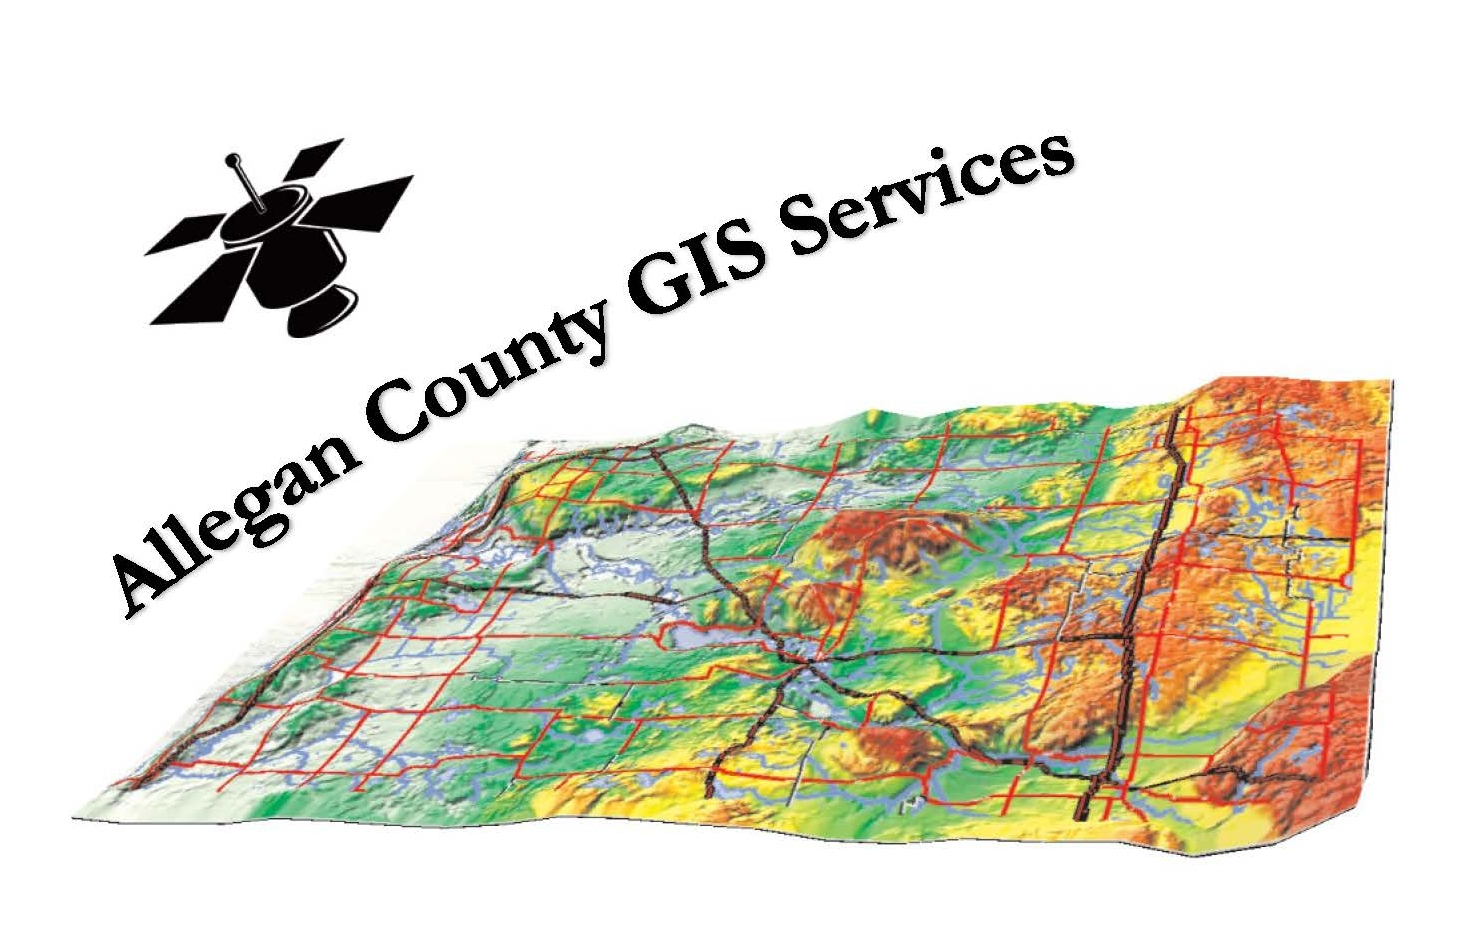
\includegraphics[scale=.45]{GIS_Logo_better.jpg}
\end{center}
\end{figure}
\Huge \bfseries \titlename \\ % Title text
\HRule \\[.4cm] % Horizontal Line added
\author{\Large Allegan County GIS \\\Large www.allegancounty.org/gis} % defines author
}  % inputs common title
\setcounter{tocdepth}{5}  % subparagraph and down
\begin{document}% document begins

\ifstandalone
\maketitle % creates title page
\clearpage
\tableofcontents % creates TOC
\clearpage
\fi

\subsection{Forfeiture Data Collection}

\subsubsection{Problem and Analysis}

\paragraph{Background}
Treasurer department has an annual responsibility to properly document the tax forfeiture process.  The LIS Department built an application in MS Access and MapInfo that consumed a daily export from BSA and was deployed to the field on a laptop.  A digital camera was used for site photos and later imported into the laptop.

\paragraph{Statement of Problem}
Current Tax Forfeiture workflow is built on MapInfo software which has been replaced by ESRI software.  The Forfeiture data collection application must be recreated in the ESRI framework.


\paragraph{Analysis}
Tax Forfeiture Application will facilitate:

\begin{itemize} %1

\item Mobile data collection on handheld device via Collector for ArcGIS configured with Allegan County GIS Portal  (\textbf{device app})

\begin{itemize} %2

\item Device app will:

\begin{itemize} %3

\item Synchronize with data in the office (online)
\item Navigate to forfeiture sites (offline)
\item Collect data and photos of forfeiture sites (offline)
\item Synchronize the collected data with data in the office (online)
\end{itemize} %3

\end{itemize} %2

\item Daily form production and printing for each site visited with required data and images.

\end{itemize} %1

\clearpage
\subsubsection{Design}

\paragraph{Overview}The Forfeiture Data Collection Application uses BSA, ArcGIS Desktop, ArcGIS Collector for Android, and ArcGIS Portal web maps and apps to enable forfeiture data collection.  A daily routine is supported that maintains forfeiture parcel data through the notification period.
\begin{center}
    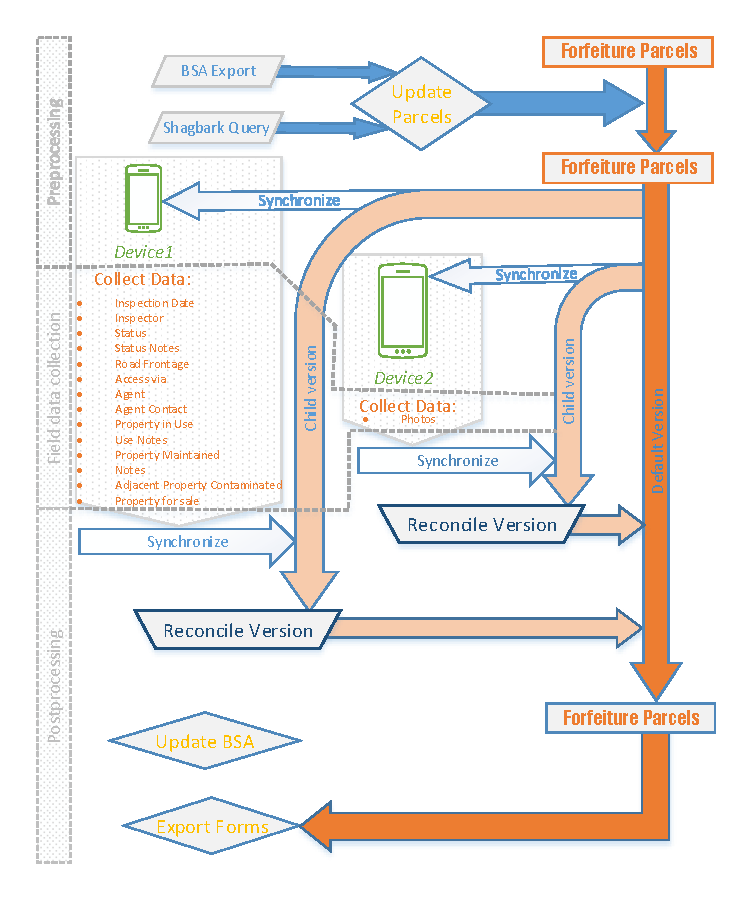
\includegraphics[width=1\textwidth]{DesignFlowChart}
    \captionof{figure}{Project Design}
    \label{img:dflow1}
\end{center}


\subparagraph{BSA data export}Details of parcels in the forfeiture process are managed in BSA Delinquent Tax.net.  The Treasurer office has a BSA export the parcels that need a site visit.  Export of the updated list is the beginning of the daily routine in this workflow.

\subparagraph{ArcGIS Desktop tasks}Tools are designed to preprocess and postprocess forfeiture parcel data for fieldwork.  The user will execute a preprocess script tool that prepares the data for field deployment.  After fieldwork, a post process script tool syncronizes data from the fieldwork with the live data on the Allegan County network. 

\subparagraph{ArcGIS Collector}A free mobile application developed and tested on Android is deployed to the field for data collection.  The application is configured to work offline(without an internet or cellular connection) by syncronizing before and after fieldwork.

\subparagraph{ArcGIS Portal Webmaps and Apps}Live data from a publishing (replica of ACPro) enterprise geodatabase (ACPub) running on SQL Server database server (acintsql01) is provided through a feature service (REST service)  named TaxReversionParcels.  A webmap called Forfeiture Field Map consumes the TaxReversionParcels feature service exposing the forfeiture parcels, for editing.  The Forfeiture Field Map is configured to work in the ArcGIS Collector App.  The app downloads the webmap, allowing the user to collect the necessary information on each forfeiture parcel in the field disconnected and uploads the changes when reconnected. 

\paragraph{Forfeiture Data Collection}

Three parts of the daily routine:
\begin{enumerate}
\item Pre-processing (in the office):

\begin{itemize}
\item Export current forfeiture list from BSA
\item Update webmap layers with results from BSA export
\item Synchronize from webmap layers to field collection device \textbf{(device app)}
\end{itemize}

\item Field data collection with device app:

\begin{itemize}
\item Support navigation to forfeiture sites
\item Provide a checklist of data points about the site
\item Attach photos to the site
\item Save results for synchronization in post-processing
\end{itemize}

\item Post-processing (in the office)

\begin{itemize}
\item Synchronize data and images collected in device app to webmap layers

\end{itemize}
\end{enumerate}

\paragraph{Backend data details}
\subparagraph{Location of production data}

\begin{center}
    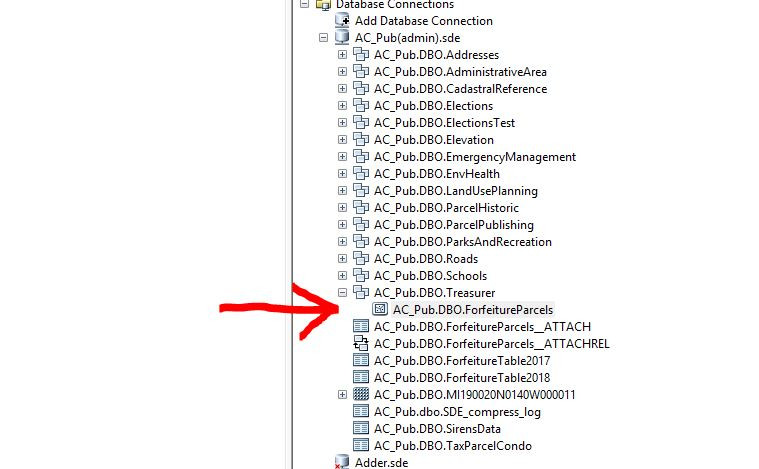
\includegraphics[width=1\textwidth]{ForfParcelsCatalog2}
    \captionof{figure}{live data}
    \label{img:forfCat1}
\end{center}

\subparagraph{ForfeitureParcels feature class}

%\begin{center}
%    \includegraphics[width=1\textwidth]{xxx}
%    \captionof{figure}{data details}
%    \label{img:fcdetails}
%\end{center}

\paragraph{Collector for ArcGIS}



\paragraph{Webmap details}

\clearpage




\subsubsection{Hard Copy Record}
\clearpage
\



\subsubsection{User Manual}

\paragraph{Admin Tasks}

\subparagraph{Setup Users in ArcGIS}Users that will run Pre and Post processing scripts must be created and given priviliges on ACPub Treasurer Feature Data Set.

\subparagraph{Setup users in Portal for ArcGIS}Users that will use the Collector for ArcGIS must have profiles added to and managed in the Allegan County GIS Portal site.


\paragraph{Collector Setup Details}

\subparagraph{Install Collector for ArcGIS}
\begin{itemize}
\item Available from the Google Play Store
\end{itemize}
\subparagraph{Configure Collector}
\begin{itemize}
\item Connect to Allegan County GIS

\begin{itemize}
\item Choose or add the connection:

\begin{verbatim}
https://gis.allegancounty.org/portal_webadaptor
\end{verbatim}

\begin{center}

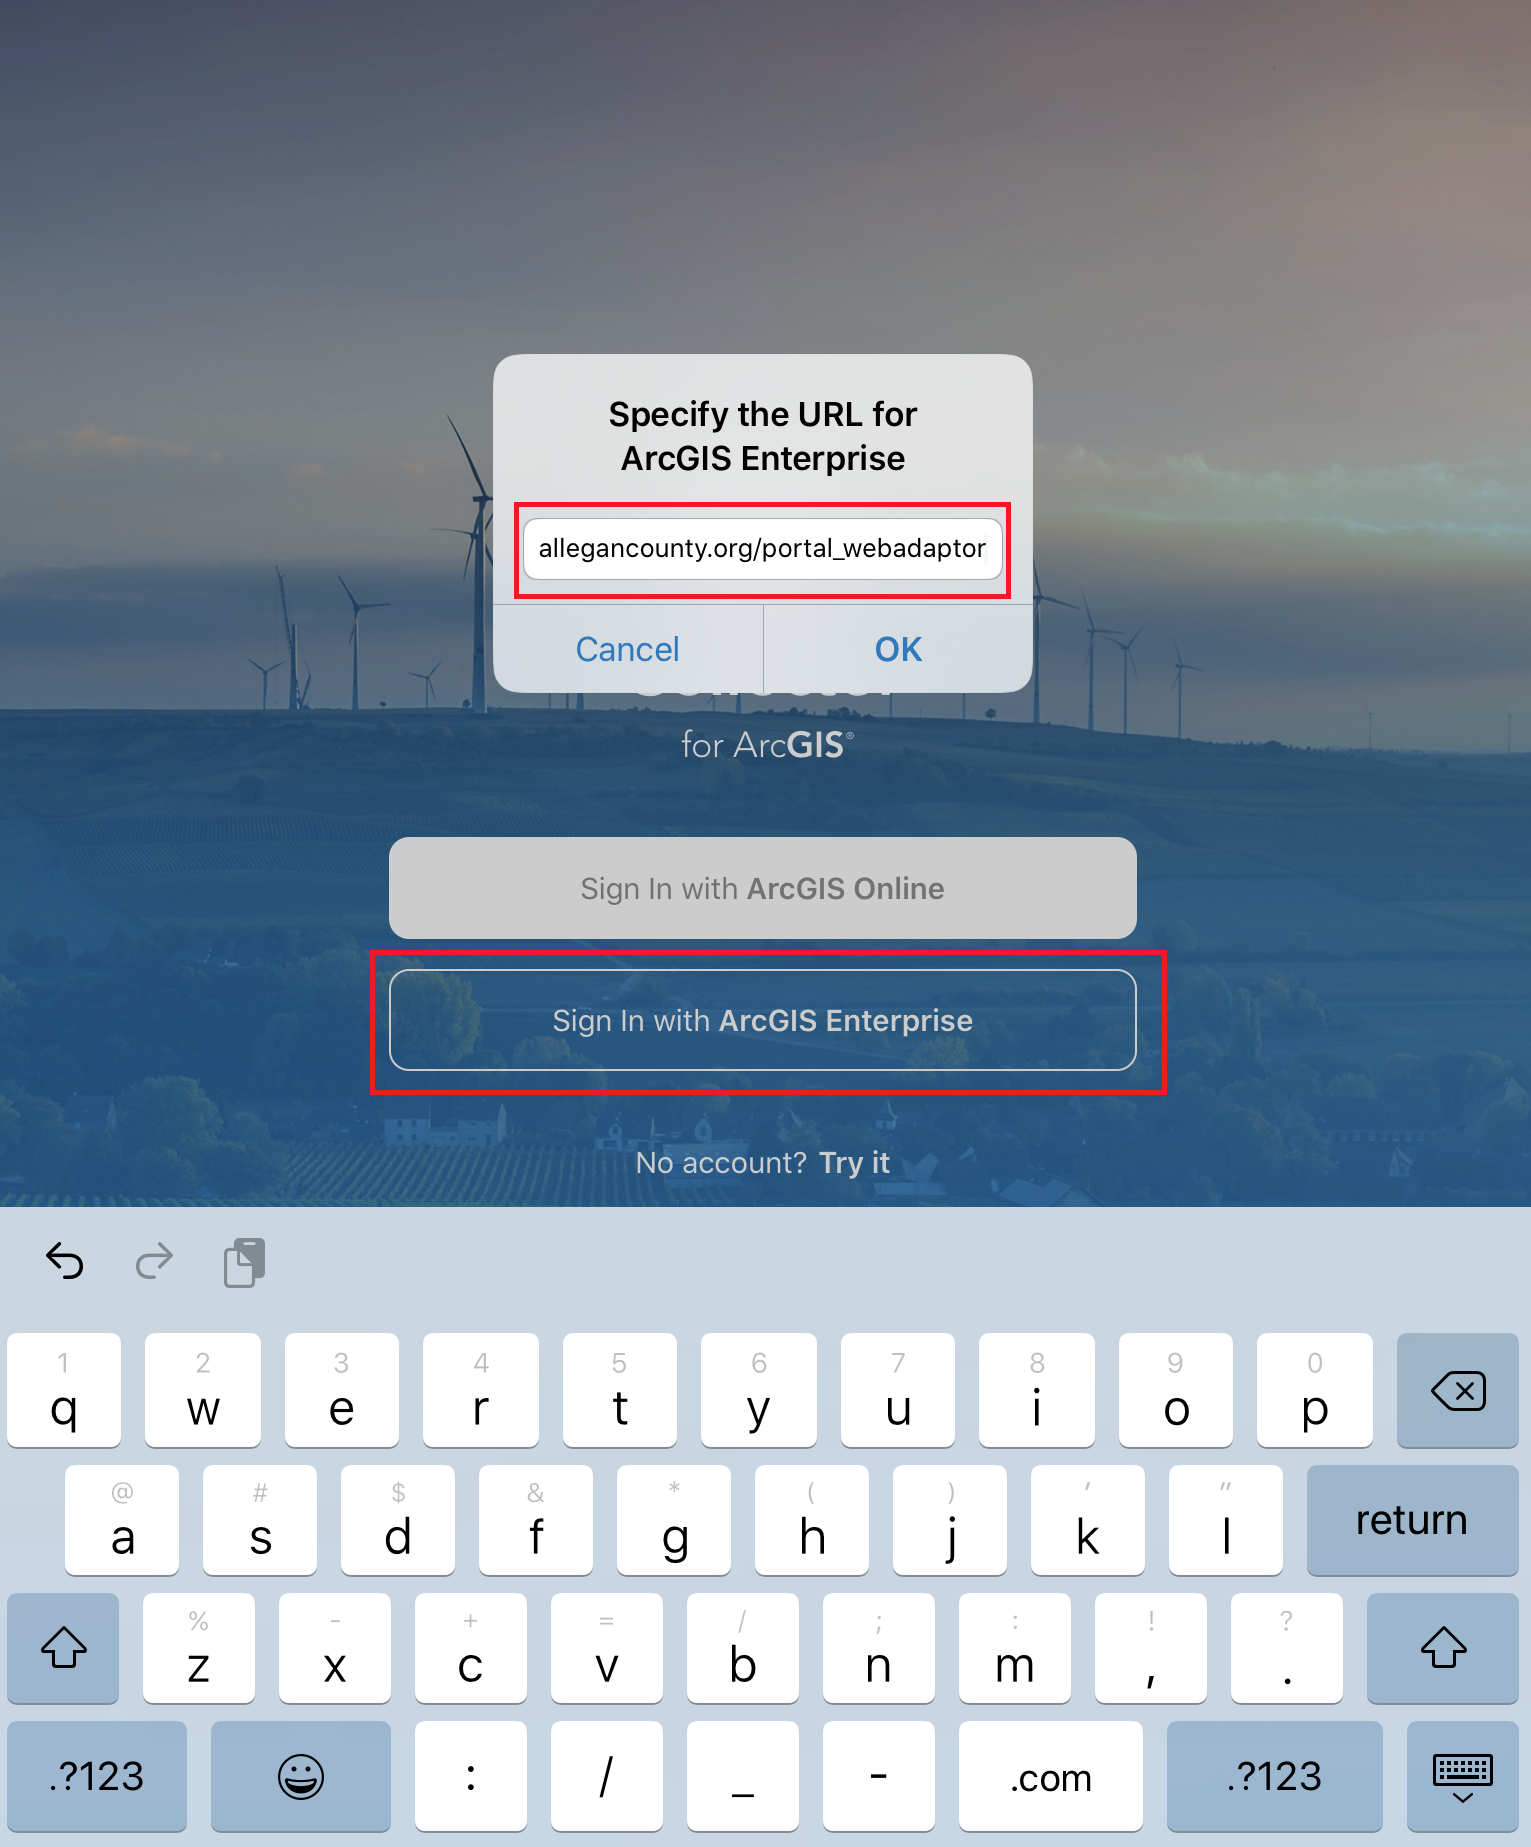
\includegraphics[width=1\textwidth]{CollectorConnection}
\captionof{figure}{Collector Connection}
%label{img:g}
\end{center}

\item Username is JMorris or CAndress
\item Password: (enter password)

\end{itemize}

\item Find the map Forfeiture Field Map under Treasury Services
\item Download the field map
\item Select area needed and detail needed and download the webmap

\end{itemize}


%\paragraph{Preprocess Before Fieldwork}

\paragraph{Daily Preprocessing Routine}

\subparagraph{Execute Preprocessing Script}A tool in ArcGIS that:

\begin{itemize}

\item Exports current forfeiture list from BSA
\item Updates webmap layers with results from BSA export

%Insert screenshot of Preprocesing script in Arc here

\end{itemize}

\subparagraph{Synchronize Webmap}In Collector for ArcGIS, push the sync button on the Forfeiture Field Map 

\paragraph{Forfeiture Data Collection}

\subparagraph{Navigation}Either device can be used to search for parcels and navigate to them. 

\subparagraph{Device 1 Field Operation}In the Forfeiture Field Map, for each site visited, select the desired parcel, push the edit button and collect the following attributes.  Save at the end of each parcel collection:
\begin{table}[h!]

\begin{center}
\begin{tabular}{l|c|r}
Field Name&Entry Type&Note\\ \hline
Property Number&Prefilled&NA\\
Inspection Date&{\footnotesize Autofill or Dropdown}&NA\\
Inspector&Dropdown&NA\\
Class&Prefilled&Missing!\\
Acres&Prefilled&Missing!\\
Address&Prefilled&NA\\
Status&Dropdown&NA\\
Status Notes&Open entry&254 Character limit\\
Road Frontage&Dropdown&Yes or No\\
Access via&Open entry&30 Character Limit\\
Agent&Open entry&30 Character Limit\\
Agent Contact&Open entry&30 Character Limit\\
Property in use&Dropdown&Yes or No Missing!\\
Use Notes&Open entry&254 Character limit\\
Property Maintained&Dropdown&Yes or No Missing!\\
Notes&Dropdown&254 Character Limit(maintNotes!)\\
Property Contaminated&Dropdown&Yes or No Missing!\\
Notes&Open entry&254 Character limit Missing!\\
Adjacent Property Contaminated&Dropdown&Missing!\\
Notes&Open entry&254 Character limit Missing!\\
Property for sale&Dropdown&Yes or No\\
Posted&Prefilled&Handled in Pre and Postprocessing\\
InList&Prefilled&Handled in Preprocessing\\
PostedInList&Prefilled&Handled in Preprocessing\\
Print Today&Dropdown&Yes or No\\

\end{tabular}
\end{center}
\end{table}


%\begin{description}[labelindent=1cm]
%
%\item [Inspection Date] Autofill current or enter other
%
%\end{description}


\subparagraph{Device 2 Field Operation}In the Forfeiture Field Map, for each site visited, select the desired parcel, push the edit button and then the add attachment button.  Select photo, and take a photo.

\paragraph{Daily Postprocessing Routine}Back at the office

\begin{description}
\item [Sync Edits] \blindtext
\item [reconcile Versions] \blindtext
\item[Print forms for site visits] \blindtext
\item[Update BSA] \blindtext
\end{description}

\clearpage
\subsubsection{Software}
\paragraph{ESRI Licensed Products}
\subparagraph{ArcDesktop}

\subparagraph{Enterprise ArcGIS Deployment}

\subparagraph{Collector for ArcGIS}Developed and tested on Android(7.0)

\end{document}